%!TEX encoding = UTF-8

\chapter{Human Perception of Robot Gestures}
\label{chap:human_perc_robotgest}

In this appendix, we study the \emph{social attitude perceived by humans when a humanoid robot moves its body parts, with no facial expressions involved}\footnote{In a previous version of this work we referred to ``emotions''~\cite{saponaro:2011:hri}, but we now use a broader expression: ``social attitudes'', in the sense of social states of mind. The reason for this change is that ``emotions'' typically refer to anger, disgust, fear, happiness, sadness, and surprise~\cite{ekman:1972}. The social attitudes that we consider are: agreement, anger, distraction, approval, and disapproval.}.

We conduct a human experiment in which human subjects are sitting in front of the iCub robot (see Sec.~\ref{sec:platform:icub}), they observe it while it performs pre-programmed head and arm movements, and they respond to a questionnaire. We select the questions in such a way that they are not boring or repetitive by using a machine learning algorithm based on the idea of active learning (i.e., an algorithm that actively chooses the data from which it learns). We report our motivation in terms of robot gesture design, our findings regarding the expressiveness of robot motion according to humans, and we propose an automated system to conduct this type of studies in a way that keeps the time devoted to making questions to humans to a minimum, while maximizing the information acquired for statistical purposes and robot gesture design.

A note on terminology: in this appendix,
(i)~we call \emph{parameters} the numerical terms associated to robot gestures types (i.e., the variables controlling joint positions, velocities and timings, as listed in Tables~\ref{tab:gesture_params:nod}--\ref{tab:gesture_params:thumbs_up-thumbs_down});
(ii)~we call \emph{parameterized gestures} the combinations of gesture types, parameters and corresponding values (i.e., \gestparval{} tuples, see Sec.~\ref{sec:parameterization}).
However, (iii)~we call \emph{weights} the \ac{BN} probabilies which specify the \acp{CPD} associated to the network.
Those weights are usually called ``parameters'' in Bayesian learning literature~(see Sec.~\ref{sec:background:theory} and~\cite{tong:2000,bishop:prml,pearl:1988:probabilistic}), but in this appendix we avoid using that term to prevent confusion with our specific meaning of robotic gesture parameters. \label{terminology_parameter_weight}

This appendix is the subject of the following publication:
\listPublicationsAppendixHumanPercRobotGest

The outline of this appendix is as follows:
Sec.~\ref{sec:human_perc_robotgest:background} provides motivational considerations and related works for the study in this appendix.
Sec.~\ref{sec:human_perc_robotgest:approach} illustrates the proposed approach.
Sec.~\ref{sec:human_perc_robotgest:results} reports the results, and
Sec.~\ref{sec:human_perc_robotgest:conclusions} draws the conclusions.

\section{Background and Related Work}
\label{sec:human_perc_robotgest:background}

\begin{figure}
\includegraphics[width=0.9\textwidth]{iCub_300px-Face.jpg}
\caption{A set of iCub facial expressions using eye LEDs, mouth LEDs and eyelid motors.}
\label{fig:iCub_facial_expressions}
\end{figure}

While the iCub robot has been used to display some basic emotional social states \cite{barros:2015:humanoids,raffard:2016:schizophrenia,pacella:2017:emotions}, this task has been mainly concerned with the robot \emph{face} by controlling its eyebrow LEDs, mouth LEDs and eyelid servomotors as shown in Fig.~\ref{fig:iCub_facial_expressions}: all features that are indeed extremely informative for the transmission of feelings. By contrast, we intend to explore the social capabilities of \emph{joint movements} located in the head, neck, torso and arms of the robot, and how human users interpret these movements when face expressions are disabled. We deliberately do \emph{not} exploit the facial features of the robot, because face to face interaction, being the chief interaction modality for humans, would be too informative: using robot facial expressions drives and biases the perception of the other's features, such as the movements, so we choose to turn off the facial expressions, giving the robot face a neutral look, as in Fig.~\ref{fig:iCub_no_face}.

\begin{figure}
\includegraphics[width=0.6\textwidth]{iCub_no_face.jpg}
\caption[The iCub face in a neutral position, without facial expressions.]{The iCub face in a neutral position, without facial expressions, as it was used during the human study of Sec.~\ref{sec:human_perc_robotgest:approach}.}
\label{fig:iCub_no_face}
\end{figure}

Our source of inspiration for transmitting social attitudes with movement while disregarding the face, is \emph{puppetry}~\cite{li:2011:ijsr}. Based on literature related to communicative robot body movements designed by puppeteers, we build a library of robot gestures with their expected attitude value (ground truth). We then model a mapping between robot movements and social attitudes perceived by humans, as a multinomial distribution.

With this setup, we ask people to attribute social attitudes ratings to robot movements. The answers are used to update the \gestatt{} matches. In addition, we employ active learning to conduct the study in a way that minimizes time and maximizes the information gain. This framework gives the system the ability to inquire about movements that are ambiguous, showing them and getting feedback more often than easily-perceived ones.

In the context of social robotics, we now review literature concerned with the perceived value associated to \emph{body gestures} and movement, in order to assess the clarity and the effectiveness of the iCub body gestures that we show to laypeople with the method explained in Sec.~\ref{sec:human_perc_robotgest:approach}.

The role of body expressions in \emph{affective \hri{}}, and more generally in affective computing, has been the subject of several studies: for a comprehensive review, we refer the reader to~\cite{kleinsmith:2013:survey}. Body movements are powerful means for conveying social attitudes, and they also facilitate multimodal interaction in which they assume other functions besides being mere gestures or controllers: for instance, in whole-body videogames with Microsoft Kinect, PlayStation Move or Nintendo Wii, movements capture and affect our own performance in the game~\cite{bianchi:2013:hci}. The information contained in body gestures can be incorporated into many applications, ranging from security and surveillance, to law enforcement, entertainment, videogames, education, and health care: for example, during rehabilitation exercises, certain specific movements and postural patterns inform clinical practitioners about the emotional conflict in the patients, and their (im)possibility to relax.

As far as the iCub robot is concerned, it has been used in specific \hri{} studies focusing on the role of certain modalities like gaze~\cite{boucher:2012:fnbot} or touch~\cite{argall:2010:icdl} during interactions.
It has been used to display basic emotions with its face (Ekman's Six Basic Emotions~\cite{ekman:1972} as shown in Fig.~\ref{fig:iCub_facial_expressions}: anger, disgust, fear, happiness, sadness, surprise).
To the best of our knowledge, the iCub has not been used to study the social attitude value carried by gestures and movement, which we will do in the remainder of this appendix.

Li and Chignell~\cite{li:2011:ijsr} have researched the social attitude understanding of robot gestures by human users, in particular by comparing robot gesture movements designed by common people versus those designed by \emph{puppeteers}, and asking users whether they perceived one of many social states of mind. The intuition is that puppetry artists are able to create engaging and communicative personalities merely by manipulating the kinematics of puppet figures. We apply the same methodology with the iCub robot.

\section{Proposed Approach}
\label{sec:human_perc_robotgest:approach}

\begin{figure}
\centering
\includegraphics[width=0.9\textwidth]{hri2011_diagram}
\caption[Block diagram of the proposed approach to study the matches between robot gestures and perceived social attitude in humans.]{Block diagram of the proposed approach to study the matches between robot gestures and perceived social attitude in humans. The library of gestures is pre-programmed (see Table~\ref{tab:robot_gestures}); the questionnaire is a multiple-scale Likert one; the scores are numbers corresponding to the Likert answers, and they are used by the Active Learning block to update an internal matrix of matches and select which robot gestures should be shown next.}
\label{fig:human_perc_robotgest:diagram}
\end{figure}

We design a library of robot gestures (without using facial expressions) and we survey a number of people about what social attitude they perceive when a humanoid robot performs such gestures. We study the results and draw conclusions about which robot movements are clear and which are not, looking at the attitude scores attributed by human subjects to robot gestures.

Recall that we conduct the human study in such a way that minimizes the time necessary for the interview sessions (as well as the robot usage, preventing breakage of delicate robot parts and consequent downtime) by employing an active learning technique, which processes the human scores attributed to the robot gestures, and decides which of the gestures require more corrections and further human feedback information: accordingly, the chosen gestures is shown, in order to maximize the information of the matches from robot gestures to perceived social attitudes, modeled as probabilistic mappings with a \acl{BN}.

As we make the robot perform the gestures and we ask human users to attribute scores about the perceived attitudes, we address two key issues related with robot gestures: (i)~whether simple robot gestures, in the absence of facial cues, convey the expected attitudes to viewers; (ii)~what contextual and motion characteristics aid gesture understanding the most~\cite{li:2011:ijsr}.

We now illustrate the details of the proposed approach.

\subsection{Design of Basic Robot Gestures}

\begin{table}
\centering
\caption[Library of robot gestures.]{Library of robot gestures, ordered by a sequential index, each one corresponding to an expected social attitude (ground truth according to the robot designer).}
\begin{tabular}{*{3}{l}} % left-aligned columns
\toprule
Gesture& \emph{Name}: description                            & Expected \\
type   &                                                     & social attitude \\
index  &                                                     & (ground truth) \\
\midrule
$T=1$  & \emph{nod}: head tilts up and down                  & agreement \\
$T=2$  & \emph{punch}: rapidly extend fist in front of robot & anger \\
$T=3$  & \emph{look out}: abruptly deviate robot head and    & distraction \\
       & gaze to a side                                      & \\
$T=4$  & \emph{thumbs up}: show fist and move thumb up       & approval \\
$T=5$  & \emph{thumbs down}: show fist and move thumb down   & disapproval \\
\bottomrule
\end{tabular}
\label{tab:robot_gestures}
\end{table}

\begin{figure}
\centering
\subfloat
{\includegraphics[width=\myWidthHumanPercRobotGestAppendix\columnwidth]{icub_nod_frame01}} \quad
%
\subfloat
{\includegraphics[width=\myWidthHumanPercRobotGestAppendix\columnwidth]{icub_nod_frame02}} \quad
%
\subfloat
{\includegraphics[width=\myWidthHumanPercRobotGestAppendix\columnwidth]{icub_nod_frame03}} \quad
%
\subfloat
{\includegraphics[width=\myWidthHumanPercRobotGestAppendix\columnwidth]{icub_nod_frame04}} \\
%
\subfloat
{\includegraphics[width=\myWidthHumanPercRobotGestAppendix\columnwidth]{icub_nod_frame05}} \quad
%
\subfloat
{\includegraphics[width=\myWidthHumanPercRobotGestAppendix\columnwidth]{icub_nod_frame06}} \quad
%
\subfloat
{\includegraphics[width=\myWidthHumanPercRobotGestAppendix\columnwidth]{icub_nod_frame07}} \quad
%
\subfloat
{\includegraphics[width=\myWidthHumanPercRobotGestAppendix\columnwidth]{icub_nod_frame08}}
\caption[Temporal snapshots of the iCub \emph{nod} gesture.]{Temporal snapshots of the iCub \emph{nod} gesture. Video available at \url{https://youtu.be/w0uvGzmTkQM}}
\label{fig:nod}
\end{figure}

\begin{figure}
\centering
\subfloat
{\includegraphics[width=\myWidthHumanPercRobotGestAppendix\columnwidth]{icub_punch_frame01}} \quad
%
\subfloat
{\includegraphics[width=\myWidthHumanPercRobotGestAppendix\columnwidth]{icub_punch_frame02}} \quad
%
\subfloat
{\includegraphics[width=\myWidthHumanPercRobotGestAppendix\columnwidth]{icub_punch_frame03}} \quad
%
\subfloat
{\includegraphics[width=\myWidthHumanPercRobotGestAppendix\columnwidth]{icub_punch_frame04}} \\
%
\subfloat
{\includegraphics[width=\myWidthHumanPercRobotGestAppendix\columnwidth]{icub_punch_frame05}} \quad
%
\subfloat
{\includegraphics[width=\myWidthHumanPercRobotGestAppendix\columnwidth]{icub_punch_frame06}} \quad
%
\subfloat
{\includegraphics[width=\myWidthHumanPercRobotGestAppendix\columnwidth]{icub_punch_frame07}} \quad
%
\subfloat
{\includegraphics[width=\myWidthHumanPercRobotGestAppendix\columnwidth]{icub_punch_frame08}}
\caption[Temporal snapshots of the iCub \emph{punch} gesture.]{Temporal snapshots of the iCub \emph{punch} gesture. Video available at \url{https://youtu.be/9pL28w1juaU}}
\label{fig:punch}
\end{figure}

\begin{figure}
\centering
\subfloat
{\includegraphics[width=\myWidthHumanPercRobotGestAppendix\columnwidth]{icub_lookout_frame01}} \quad
%
\subfloat
{\includegraphics[width=\myWidthHumanPercRobotGestAppendix\columnwidth]{icub_lookout_frame02}} \quad
%
\subfloat
{\includegraphics[width=\myWidthHumanPercRobotGestAppendix\columnwidth]{icub_lookout_frame03}} \quad
%
\subfloat
{\includegraphics[width=\myWidthHumanPercRobotGestAppendix\columnwidth]{icub_lookout_frame04}} \\
%
\subfloat
{\includegraphics[width=\myWidthHumanPercRobotGestAppendix\columnwidth]{icub_lookout_frame05}} \quad
%
\subfloat
{\includegraphics[width=\myWidthHumanPercRobotGestAppendix\columnwidth]{icub_lookout_frame06}} \quad
%
\subfloat
{\includegraphics[width=\myWidthHumanPercRobotGestAppendix\columnwidth]{icub_lookout_frame07}} \quad
%
\subfloat
{\includegraphics[width=\myWidthHumanPercRobotGestAppendix\columnwidth]{icub_lookout_frame08}}
\caption[Temporal snapshots of the iCub \emph{look out} gesture.]{Temporal snapshots of the iCub \emph{look out} gesture. Video available at \url{https://youtu.be/RJIx27xHJ34}}
\label{fig:lookout}
\end{figure}

\begin{figure}
\centering
\subfloat
{\includegraphics[width=\myWidthHumanPercRobotGestAppendix\columnwidth]{icub_thumbsup_frame01}} \quad
%
\subfloat
{\includegraphics[width=\myWidthHumanPercRobotGestAppendix\columnwidth]{icub_thumbsup_frame02}} \quad
%
\subfloat
{\includegraphics[width=\myWidthHumanPercRobotGestAppendix\columnwidth]{icub_thumbsup_frame03}} \quad
%
\subfloat
{\includegraphics[width=\myWidthHumanPercRobotGestAppendix\columnwidth]{icub_thumbsup_frame04}} \\
%
\subfloat
{\includegraphics[width=\myWidthHumanPercRobotGestAppendix\columnwidth]{icub_thumbsup_frame05}} \quad
%
\subfloat
{\includegraphics[width=\myWidthHumanPercRobotGestAppendix\columnwidth]{icub_thumbsup_frame06}} \quad
%
\subfloat
{\includegraphics[width=\myWidthHumanPercRobotGestAppendix\columnwidth]{icub_thumbsup_frame07}} \quad
%
\subfloat
{\includegraphics[width=\myWidthHumanPercRobotGestAppendix\columnwidth]{icub_thumbsup_frame08}}
\caption[Temporal snapshots of the iCub \emph{thumbs up} gesture.]{Temporal snapshots of the iCub \emph{thumbs up} gesture. Video available at \url{https://youtu.be/ZHN91AN1t_o}}
\label{fig:thumbsup}
\end{figure}

\begin{figure}
\centering
\subfloat
{\includegraphics[width=\myWidthHumanPercRobotGestAppendix\columnwidth]{icub_thumbsdown_frame01}} \quad
%
\subfloat
{\includegraphics[width=\myWidthHumanPercRobotGestAppendix\columnwidth]{icub_thumbsdown_frame02}} \quad
%
\subfloat
{\includegraphics[width=\myWidthHumanPercRobotGestAppendix\columnwidth]{icub_thumbsdown_frame03}} \quad
%
\subfloat
{\includegraphics[width=\myWidthHumanPercRobotGestAppendix\columnwidth]{icub_thumbsdown_frame04}} \\
%
\subfloat
{\includegraphics[width=\myWidthHumanPercRobotGestAppendix\columnwidth]{icub_thumbsdown_frame05}} \quad
%
\subfloat
{\includegraphics[width=\myWidthHumanPercRobotGestAppendix\columnwidth]{icub_thumbsdown_frame06}} \quad
%
\subfloat
{\includegraphics[width=\myWidthHumanPercRobotGestAppendix\columnwidth]{icub_thumbsdown_frame07}} \quad
%
\subfloat
{\includegraphics[width=\myWidthHumanPercRobotGestAppendix\columnwidth]{icub_thumbsdown_frame08}}
\caption[Temporal snapshots of the iCub \emph{thumbs down} gesture.]{Temporal snapshots of the iCub \emph{thumbs down} gesture. Video available at \url{https://youtu.be/AKvA6lIt25Q}}
\label{fig:thumbsdown}
\end{figure}

Because we are interested in mapping simple robot gestures to social attitudes that we wish to transmit successfully, the first crucial aspect of the work consists in \emph{designing a library of basic robot motions} which do not rely on facial information, and their expected perceived attitudes.
We do this design task manually, i.e., a set of precise robot gestures and joint trajectories are pre-programmed by hand, modulating the available joint positions and timings, using the iCub kinematic structure (\url{http://wiki.icub.org/wiki/ICub_joints}) and evaluating the resulting movements qualitatively (this process being repeated a number of times).
In order to actuate the robot joints, we use the position-based control, the Cartesian Interface~\cite{pattacini:2010:iros} and the Gaze Interface~\cite{roncone:2016:rss}, all available in the iCub software repository (\url{http://www.icub.org}).
The end result of this process is summarized in Table~\ref{tab:robot_gestures}, which lists the designed gestures with corresponding numerical identifiers, names, verbal descriptions and, importantly, an expected attitude ground truth value.
Recall that the main objective of this work is to study the match between robot gestures~($A$) and human-perceived social attitudes~$(E)$.

Each of the designed gesture types, listed in the first column of Table~\ref{tab:robot_gestures}, consists of a trajectory computed between two or more points in space (either joint space or Cartesian space, depending on the gesture being designed) with adjusted velocities and timings between the points to interpolate.
We show
the \emph{nod} robot gesture in Fig.~\ref{fig:nod},
the \emph{punch} robot gesture in Fig.~\ref{fig:punch},
the \emph{lookout} robot gesture in Fig.~\ref{fig:lookout},
the \emph{thumbs up} robot gesture in Fig.~\ref{fig:thumbsup}, and
the \emph{thumbs down} robot gesture in Fig.~\ref{fig:thumbsdown}.
The main issue encountered during the interpretation of the gestures by interviewees was about the \emph{punch} gesture: this gesture looked ambiguous, likely because the fist was not completely closed.

\subsection{Parameterization of Robot Gestures}
\label{sec:parameterization}

The robot gestures that we study are divided into a few basic types~$T$, as listed in Table~\ref{tab:robot_gestures}. However, to have greater flexibility while displaying robot gestures as well as during the machine learning phases, we enrich the model with a set of specific parameters~$P$ (different for each gesture type) that modulate the appearance of robot gestures, listed explicitly in Tables~\ref{tab:gesture_params:nod}--\ref{tab:gesture_params:thumbs_up-thumbs_down}. Each of the parameters takes a discrete value from a set~$V$ (different for each \gestpar{} pair), which can be seen as a histogram (e.g., a velocity-like parameter value range can be divided into a low-velocity bin~$v_1$, a medium-velocity bin~$v_2$ and a high-velocity bin~$v_3$).

As a result, in the general formulation of our framework described below, the matches (\acl{BN} weights) are between \gestparval{} tuples (rows) and perceived attitudes (columns). This means that the number of rows can potentially be much larger than the number of columns: active learning is especially useful in these scenarios, being able to select a query (row) among many of them, according to a probabilistic criterion. Even though our formalism is quite general, in the experimental results (Sec.~\ref{sec:human_perc_robotgest:results}) we will make some simplifying assumptions as to the number of parameters and values.

\begin{table}
\centering
\caption{Parameters of the ``nod'' gesture.}
\begin{tabular}{*{3}{l}} % left-aligned columns
\toprule
Parameter       & Parameter         & Meaning \\
index           & symbol            & \\
\midrule
$P_1$           & $x_0^{(0)}$       & initial position of neck pitch joint \\
$P_2$           & $x_0^{(1)}$       & final position of neck pitch joint \\
$P_3$           & $\dot{x}_0$       & velocity of neck pitch joint \\
$P_4$           & $t_{(0)\to(1)}$   & time to transition from initial to \\
                &                   & final positions \\
$P_5$           & $t_{(1)\to(0)}$   & time to transition from final to \\
                &                   & final positions \\
\bottomrule
\end{tabular}
\label{tab:gesture_params:nod}
\end{table}

\begin{table}
\centering
\caption{Parameters of the ``punch'' gesture.}
\begin{tabular}{*{3}{l}} % left-aligned columns
\toprule
Parameter       & Parameter         & Meaning \\
index           & symbol            & \\
\midrule
$P_1$           & $\dot{x}_{7:15}$  & velocity of finger joints when \\
                &                   & closing hand \\
$P_2$           & $t_{(0)\to(1)}$   & time to transition arm joints from initial \\
                &                   & to final positions \\
$P_3$           & $t_{(1)\to(0)}$   & time to transition arm joints from final \\
                &                   & to initial positions \\
\bottomrule
\end{tabular}
\label{tab:gesture_params:punch}
\end{table}

\begin{table}
\centering
\caption{Parameters of the ``look out'' gesture.}
\begin{tabular}{*{3}{l}} % left-aligned columns
\toprule
Parameter       & Parameter         & Meaning \\
index           & symbol            & \\
\midrule
$P_1$           & $x_{0:2}^{(0)}$   & initial position of neck joints\\
$P_2$           & $x_{0:2}^{(1)}$   & final position of neck joints\\
$P_3$           & $\dot{x}_{0:2}$   & velocity of neck joints \\
$P_4$           & $t_{(0)\to(1)}$   & time to transition head joints from initial \\
                &                   & to final positions \\
\bottomrule
\end{tabular}
\label{tab:gesture_params:look_out}
\end{table}

\begin{table}
\centering
\caption{Parameters of the ``thumbs up'' and ``thumbs down'' gestures.}
\begin{tabular}{*{3}{l}} % left-aligned columns
\toprule
Parameter       & Parameter         & Meaning \\
index           & symbol            & \\
\midrule
$P_1$           & $x_8^{(0)}$       & initial position of thumb opposition joint \\
$P_2$           & $x_8^{(1)}$       & final position of thumb opposition joint \\
$P_3$           & $\dot{x}_8$       & velocity of thumb opposition joint \\
$P_4$           & $t_{(0)\to(1)}$   & time to transition arm joints from initial \\
                &                   & to final positions \\
$P_5$           & $t_{(1)\to(0)}$   & time to transition arm joints from final \\
                &                   & to initial positions \\
\bottomrule
\end{tabular}
\label{tab:gesture_params:thumbs_up-thumbs_down}
\end{table}

\subsection{Human Questionnaire}
\label{sec:questionnaire}

To survey human interpretation of the robot movements, we present people with a five-level Likert questionnaire (see Fig.~\ref{fig:human_perc_robotgest:diagram}). The robot displays gestures selected from the library of Table~\ref{tab:robot_gestures} according to an order which is computed online (see Sec.~\ref{sec:active_learning}), and we ask subjects to rate their level of agreement to a number of statements relative to social attitudes:
\begin{itemize}
\item ``This gesture expresses agreement.''

\item ``This gesture expresses anger.''

\item ``This gesture expresses distraction.''

\item ``This gesture expresses approval.''

\item ``This gesture expresses disapproval.''
\end{itemize}

For each displayed movement, we ask people to rate each of the above statements with a score ranging from~1 (strongly disagree) to~5 (strongly agree). For each examined \gestparval{} we thus have a vector of scores~$r_l$, where~$l = 1, \dots, L$ is the attitude index. We define the \emph{normalized Likert score} as
\begin{equation} \label{eq:normalized_likert_score}
c_l = \frac{1}{\sum_{i=1}^L r_i} r_l, \quad l = 1, \dots, L,
\end{equation}
which is a new score derived from~$r_l$, but such that the elements~$c_1, \dots, c_L$ sum to unity. For example, if a vector of scores is~$[5 \quad 1 \quad 2 \quad 4 \quad 1]$, then its normalized version is~$[5/13 \quad 1/13 \quad 2/13 \quad 4/13 \quad 1/13]$.


\subsection{Probabilistic Model of \GestAtt{} Matches}

We will now describe how to model the questionnaire scores provided by human subjects (see Sec.~\ref{sec:questionnaire}) in a \acl{BN} composed of two nodes: A~(parameterized gesture) $\to$~E (attitude).

Node~A includes a \emph{fixed} \gestparval{} tuple combining a gesture type, a gesture-specific parameter and a possible value for it, as follows: it contains the specific type of gesture $T = t_i$, where $i = 1, \ldots, M$ ($M$: number of possible gestures), as in Table~\ref{tab:robot_gestures}, its parameters values $V_{ij} = \{ v_{ijk} \}, j = 1, \ldots, P_i$ ($P_i$: number of parameters that describe gesture~$i$, as in Tables~\ref{tab:gesture_params:nod}--\ref{tab:gesture_params:thumbs_up-thumbs_down}), $k = 1, \ldots, K_{ij}$ ($K_{ij}$: number of possible values of parameter~$j$ for gesture~$i$). For notational convenience, we use a unique discrete index~$n=1, \ldots, N$ to count all the possible \gestparval{}~$3$-tuples, thus incorporating the indexes~$i, j, k$ like this:
\begin{equation} \label{eq:gestparval_index}
\begin{split}
n = 1, \ldots, \overbrace{\sum_{i=1}^M \sum_{j=1}^{P_i} K_{ij}}^N, \quad & \forall i=1,\ldots,M, \\
                                                                         & \forall j=1,\ldots,P_i, \\
                                                                         & \forall k=1,\ldots,K_{ij}.
\end{split}
\end{equation}

Node~$E$ encodes a pre-defined \emph{set} of possible attitudes $e_l$, $l = 1, \ldots, L$, corresponding to the last column of Table~\ref{tab:robot_gestures}.

The probability distribution $P(E \given A)$ is modeled as a multinomial distribution $P(E = e_l \given A = a_n) = \bm{\theta}_{ln}$, where $\theta$ are the \acl{BN} probability weights\footnote{Recall from p.~\pageref{terminology_parameter_weight} that we call \emph{weights} the \acl{BN} probabilies which specify the \acp{CPD} associated to the network. Those weights are usually called ``parameters'' in machine learning literature, but we avoid that term because we already employ it for robotic gesture parameters.}, $l$~is the attitude index, $n$~is the \gestparval{} index and $\sum_l \theta_{ln} = 1$ for each~$a_n$:
\begin{equation} \label{eq:gestatt_multinomial}
P(E \given A) =
              \begin{bmatrix}
              \theta_{11} & \cdots & \theta_{L1} \\
              \theta_{12} & \cdots & \theta_{L2} \\
              \vdots & \ddots & \vdots \\
              \theta_{1N} & \cdots & \theta_{LN}
              \end{bmatrix}.
\end{equation}

We have modeled a \acl{BN} from~$N$ multinomial tables, one for each \gestparval{}~$a_n$ (each row of the matrix in~\eqref{eq:gestatt_multinomial}), expressing the corresponding distribution of attitude perceived by human users.

Furthermore, we express each weight~$\theta_{ln}$ of~\eqref{eq:gestatt_multinomial} as a fractional expression:
\begin{equation} \label{eq:one_fractional_weight}
\theta_{ln} = \frac{s_{ln}}{\#a_n},
\end{equation}
where~$s_{ln}$ is the cumulative normalized score of attitude~$l$ to~\gestparval{} tuple~$n$ (see~\eqref{eq:normalized_likert_score}), and~$\#a_n$ is the total number of cases where \gestparval{} tuple~$n$ was shown.

We assume that the structure of the \acl{BN} is given, and we focus on estimating (updating) the weights~$\bm{\theta}$ by using data coming from human-provided social attitude scores. We keep a \ac{PDF} over possible weight values, and we assume independence between weights~\cite{tong:2000}, which allows us to represent the joint distribution~$P(\bm{\theta})$ as a set of independent multinomial distributions, one for each \gestparval{} case.

\subsection{Active Learning Algorithm}
\label{sec:active_learning}

The scores that result from the human survey described in Sec.~\ref{sec:questionnaire} are sent to an \emph{active} \acl{BN} learning program that learns (updates) the weights of the network, as proposed by~\cite{tong:2000}. In the active learning framework, the learner has the ability to guide the instances it gets, by querying for a particular input rather than proceeding randomly or sequentially from a set. In particular, in an unsupervised learning context, the system can request information in regions where the probability distribution that models the data is currently uninformative.

We will now define some quantities necessary for the algorithm, and we will describe the \emph{selection step} as well as the actual \emph{update step}, in accordance to Fig.~\ref{fig:human_perc_robotgest:diagram}.

For one \gestparval{} tuple~$a_n$ (i.e., one row of~\eqref{eq:gestatt_multinomial}), we denote its \emph{entropy} as
\begin{equation} \label{eq:entropy_prior}
H(\bm{\theta}_n) = - \sum_{l=1}^{L} \theta_{ln} \log (\theta_{ln}),
\end{equation}
where~$\log$ is the natural logarithm (the base of the logarithm does not affect the results), and~$\theta_{ln}$ is one weight of the \ac{BN} as in~\eqref{eq:one_fractional_weight} (i.e., one entry of the matrix in~\eqref{eq:gestatt_multinomial}).

The \emph{expected posterior entropy} of one~$a_n$ tuple is computed~\cite[Eq.~1]{tong:2000} by averaging the entropies that would arise from all particular choices of vectorial Likert scores ($r = 1,\ldots,R^L$, where~$L$ is the number of attitudes or elements in the vectorial scores, and~$R$ are the possible Likert levels), weighted by the probability of each choice,~$P(r)$:
\begin{align}
H'(\bm{\theta}_n) &= \sum_{r=1}^{R^L} P(r) \left( - \sum_{l=1}^L \theta_{ln}^{(r)} \log \left( \theta_{ln}^{(r)} \right) \right), \label{eq:posterior_intractable} \\
%
\theta_{ln}^{(r)} &= \frac{s_{ln} + c_{lr}}{\#a_n + 1}. \label{eq:theta_upd_intractable}
\end{align}
However,~\eqref{eq:posterior_intractable} and~\eqref{eq:theta_upd_intractable} are computationally costly due to the exponential number~$R^L$ of possible~$\bm{c}$ score choices.

During the selection step we thus make a simplifying assumption: \emph{we only consider score vectors where the answer is fully polarized to one attitude, and all the other ones are zero}. This is based on the empirical observation that our interviewed subjects generally lean towards attributing one clear attitude to a gesture, disregarding all the other ones. The benefit of this assumption is that it makes the expected posterior entropy of~\eqref{eq:posterior_intractable} tractable. As a consequence, the prior~$P(r)$ can now be taken to be the current weight value~$\theta_{ln}$ (i.e., before the update), and we can write:
\begin{align}
H''(\bm{\theta}_n) &= \sum_{r=1}^R \theta_{ln} \left( - \sum_{l=1}^L \theta_{ln}^{(r)} \log \left( \theta_{ln}^{(r)} \right) \right), \label{eq:posterior_simplified} \\
%
\theta_{ln}^{(r)} &= \frac{s_{ln} + \delta_{lr}}{\#a_n + 1}, \label{eq:theta_upd_simplified}
\end{align}
where~$\delta_{lr}$ is the Kronecker delta:
\begin{equation} \label{eq:kronecker_delta}
\delta_{lr} =
              \begin{cases}
              0 & l \neq r \\
              1 & l = r.
              \end{cases}
\end{equation}

In~\eqref{eq:posterior_simplified} and~\eqref{eq:theta_upd_simplified}, $\theta_{ln}^{(r)}$ is the ``imagined'' version of a weight (see~\eqref{eq:one_fractional_weight}), computed according to the following update rule: we multiply the previous value~$\theta_{ln}$ by the counter~$\#a_n$ (number of previous experiments with~$A=a_n$), we sum the maximum scores obtainable~(\eqref{eq:kronecker_delta}), and we divide by the incremented counter~$\#a_n + 1$.

Finally, the \emph{entropy gain} is the difference between the entropy before and after learning, or equivalentely, between the current entropy (i.e., before applying the learning step) and the expected posterior entropy after a trial~\cite[Eq.~7]{tong:2000}:
\begin{equation} \label{eq:entropy_gain}
H_{\text{gain}}(\bm{\theta}_n) = H(\bm{\theta}_n) - H''(\bm{\theta}_n).
\end{equation}

\emph{Selection step.} To select which is the most convenient parameterized gesture~$a_n^{*}$ to display from the library (i.e., which row of~\eqref{eq:gestatt_multinomial}), we measure the entropy gain of all the rows and we select the row that maximizes such quantity:
\begin{equation} \label{eq:argmax}
a_n^{*} = \argmax_n H_{\text{gain}}(\bm{\theta}_n).
\end{equation}

Rather than querying every person for the same entire sequence of robot gestures in the entire ordered database, the learner selects the next query (row~$a_n$) using probability theory in an efficient way: efficient in the sense of reduced number of queries, and reduced overall time spent doing the experiment for an interview subject. In addition to the maximization criterion of~\eqref{eq:argmax}, we also employ these heuristics:
\begin{description}
\item[No Repetitions:] we prevent the system from showing the robot gesture that it showed one iteration before;

\item[Randomization:] if there are more than one winning~$a_n^{*}$ with the same entropy gain (e.g., when starting the experiment with a uniform prior), select one of them at random.
\end{description}

\emph{Update step.} After having shown the robot performing the chosen parameterized gesture~$a_n$ to an interviewed subject, we obtain the vector of questionnaire answers, we normalize it ($\bm{c}$, see~\eqref{eq:normalized_likert_score}) and we update the weights of the model as follows:
\begin{equation} \label{eq:update_rule}
\frac{s_{ln}}{\#a_n} \leftarrow \frac{s_{ln} + c_l}{\#a_n + 1}, \quad \forall l=1,\ldots,L,
\end{equation}
where the left-hand side is the previous score~$\theta_{ln}$ (see~\eqref{eq:one_fractional_weight}).

\bigskip

The main advantage of our approach is that the \hr{} experiment session is shorter than it would be with an exhaustive search (we do not survey \emph{all} people about \emph{all} the possible $A \to E$ matches), thus making the survey relatively \emph{brief and interesting}. Other advantages are that the system focuses its effort on the most ambiguous gestures (they are repeated more often, so the main share of queries and information gathering is concentrated on them), and that, by not showing exhaustively all the robot movements to all people, we reduce the wear and tear which affects fragile robot parts (e.g., steel tendons).

\section{Experimental Results}
\label{sec:human_perc_robotgest:results}

The proposed system maintains a multinomial map from (parameterized) robot gestures to perceived human attitude, as described in Sec.~\ref{sec:human_perc_robotgest:approach}.

In the remainder of this appendix, we assume a \emph{simplification} with respect to the general formulation of Sec.~\ref{sec:parameterization}: we fix the number of parameters to be~$1$ for all gesture types, and the number of values~(discretization bins) to be~$1$ for all parameters. This restriction is imposed for practical reasons: (i)~from the machine learning perspective, to reduce the number of trials required to appreciate a learning behavior by the system, (ii)~from the robotics perspective, to reduce the usage of the robot and the number of movements, especially of the arms and hands, having observed that some metal cables can break frequently when used many times with high accelerations, causing downtime and annoyance, (iii)~from the human subjects perspective, to keep the time spent interviewing each human subject to a minimum, around~10 to~15 minutes per person, after which the possibility of the interviewee becoming bored or tired increases.

By forcing the number of gesture parameters to be equal for all gesture types ($P_i \equiv P \quad \forall i$), and the number of possible value discretization bins to be equal for all gesture parameters ($K_{ij} \equiv K \quad \forall i \quad \forall j$), the expression in~\eqref{eq:gestparval_index} that enumerates the parameterized robot gestures becomes
\begin{equation*}
n = 1, \ldots, \overbrace{\sum_{i=1}^M \sum_{j=1}^P K}^N,
\end{equation*}
where~$P$ is the set of parameters for all gesture types, and~$K$ is the set of discretized values permitted for all gesture parameters.

Furthermore, because we also impose that~$P = K = 1$, the expression further simplifies to
\begin{equation*}
n = 1, \ldots, M=N,
\end{equation*}
which means that the multinomial map of~\eqref{eq:gestatt_multinomial} now consists of a matrix with~$M$ rows and~$L$ columns, where $M$~is the number of robot gestures and~$L$ is the number of human attitudes.

Before starting the interview session, we initialize the matrix of the \acl{BN} weights (see~\eqref{eq:gestatt_multinomial} and~\eqref{eq:one_fractional_weight}) to be uniform, considering the~$5$ robot gestures and human attitudes listed in Table~\ref{tab:robot_gestures}:
\begin{equation*}
\begin{split}
P(E | A) &= \bm{\theta}_{ln} \\
         &= \frac{\bm{s}_{ln}}{\#a_n} \\
         &= \begin{bmatrix}
            0.2/1  & \cdots & 0.2/1 \\
            0.2/1  & \cdots & 0.2/1 \\
            \vdots & \ddots & \vdots \\
            0.2/1  & \cdots & 0.2/1
            \end{bmatrix},
\end{split}
\end{equation*}
where each row represents a robot gesture and each column the match of that gesture to an attitude. These initial values are visualized in Fig.~\ref{fig:gestatt:start}.

Then, we ask interviewed subjects to sit in front of the robot, to observe one robot movement (chosen online by the learner, initially randomly).
We ask users to rank each movement with social attitude scores and we feed the resulting score vector into the system.
The active learning system will then choose the next movement to display, and the process is repeated.
The matrix starts being updated as the system gets more and more answers, as shown in Fig.~\ref{fig:gestatt}.

\begin{figure}
\centering
\subfloat[][Initial matches.]
{\includegraphics[width=0.45\textwidth]{gestatt_after00_withoutNI}
\label{fig:gestatt:start} } \quad
%
\subfloat[][Matches after interviewing~1 person.]
{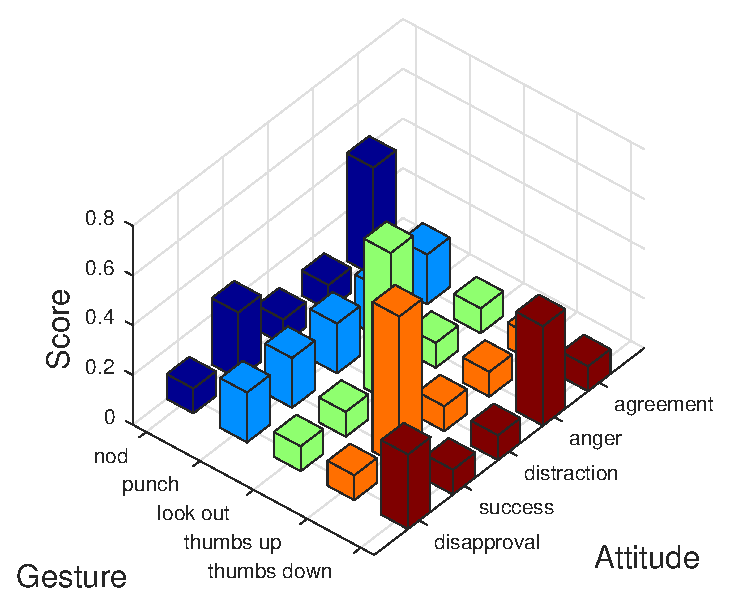
\includegraphics[width=0.45\textwidth]{gestatt_after01_withoutNI}
\label{fig:gestatt:01} } \\
%
\subfloat[][Matches after interviewing~5 people.]
{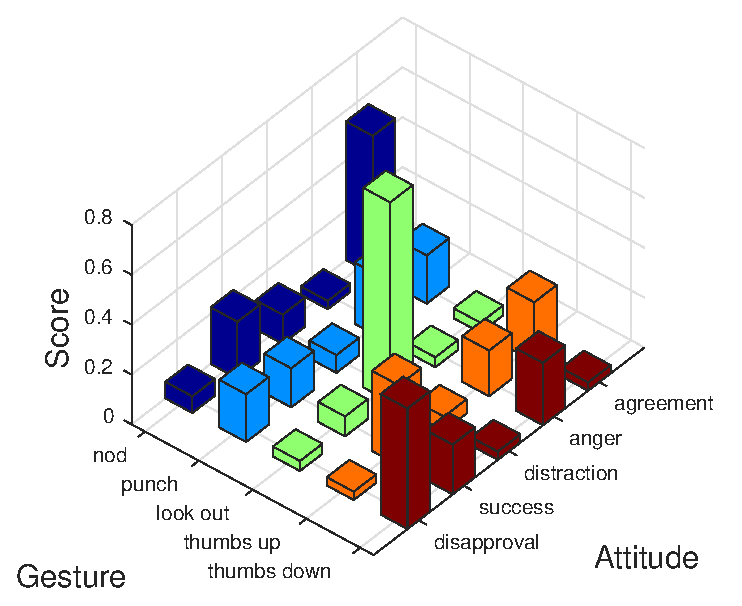
\includegraphics[width=0.45\textwidth]{gestatt_after05_withoutNI}
\label{fig:gestatt:05} } \quad
%
\subfloat[][Matches after interviewing~10 people.]
{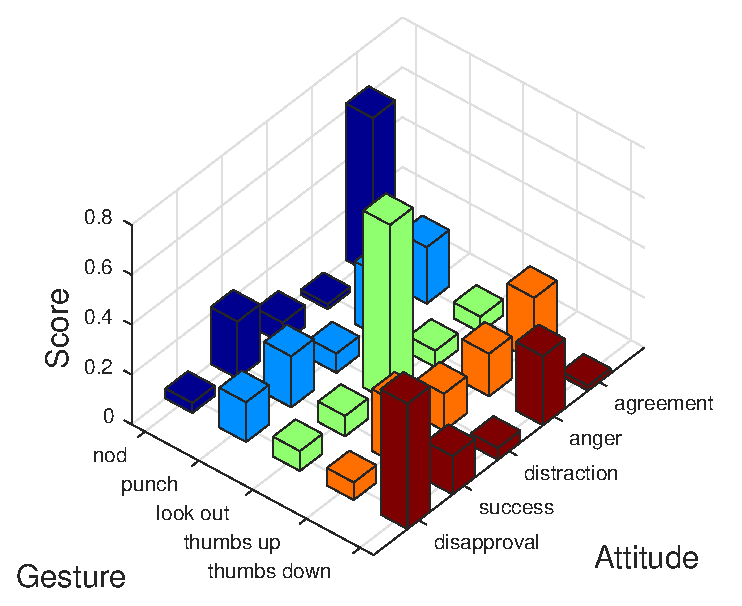
\includegraphics[width=0.45\textwidth]{gestatt_after10_withoutNI}
\label{fig:gestatt:10} } \\
%
\subfloat[][Matches after interviewing~15 people.]
{\includegraphics[width=0.45\textwidth]{gestatt_after15_withoutNI}
\label{fig:gestatt:15} } \quad
%
\subfloat[][Final matches after interviewing~20 people.]
{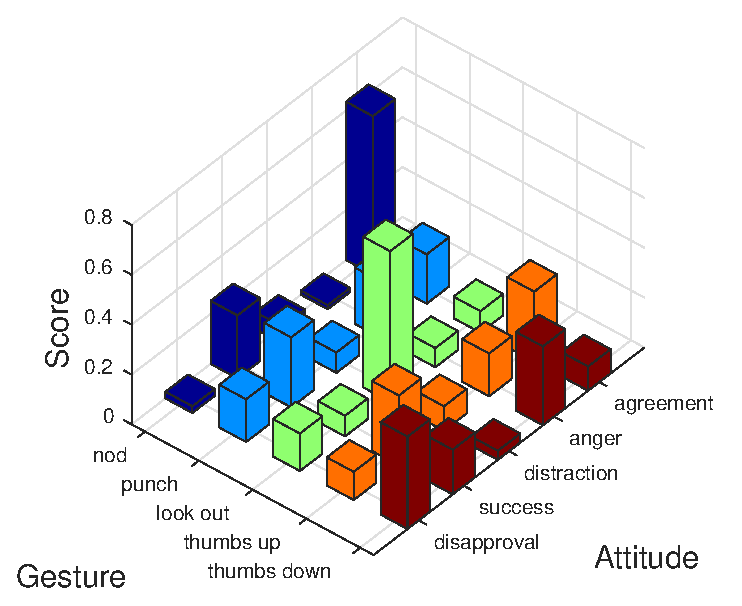
\includegraphics[width=0.45\textwidth]{gestatt_after20_withoutNI}
\label{fig:gestatt:end} }
%
\caption[Temporal evolution of the \gestatt{} matches as the human survey is carried out.]{Temporal evolution of the \gestatt{} matches as the human survey is carried out and the questionnaire answers are fed into the active learning system.}
\label{fig:gestatt}
\end{figure}

In total we survey 20~people: to each of them we show $5~(\pm 1)$ movements and in the end we obtain the mapping displayed in Fig.~\ref{fig:gestatt:end}.
It shows that gesture~1 (``nod'') was the one with the clearest \gestatt{} correspondence; it soon acquired high ``agreement'' and ``approval'' scores, i.e., the system rapidly received information about it (the gesture's expected entropy gain as in~\eqref{eq:entropy_gain} got lower) and was not bothered to query it again: it was displayed less time than the others.
This also tells us that this particular robot gesture design was good.
Gesture~3 (``look out'') also resulted in a decent ``distraction'' score.
The remaining gestures performed poorly, in fact several subjects were puzzled about them.
Possible reasons are: (i)~robot gesture design has to be improved; (ii)~the iCub humanoid does not have mechanical capabilities (e.g., accelerations are limited) to convey that attitude solely with movement (excluding facial expressions); (iii)~the questionnaire has to be adjusted, as some of the possible attitudes have an overlap, and the ground truth is too easy for people to guess.

\begin{figure}
\centering
%
\subfloat[][Initial entropies (uniform distribution).]
{\includegraphics[width=0.45\textwidth]{entropy_after00_withoutNI}
\label{fig:entropy_by_people:start} } \quad
%
\subfloat[][Entropies after interviewing~1 person.]
{\includegraphics[width=0.45\textwidth]{entropy_after01_withoutNI}
\label{fig:entropy_by_people:01} } \\
%
\subfloat[][Entropies after interviewing~5 people.]
{\includegraphics[width=0.45\textwidth]{entropy_after05_withoutNI}
\label{fig:entropy_by_people:05} } \quad
%
\subfloat[][Entropies after interviewing~10 people.]
{\includegraphics[width=0.45\textwidth]{entropy_after10_withoutNI}
\label{fig:entropy_by_people:10} } \\
%
\subfloat[][Entropies after interviewing~15 people.]
{\includegraphics[width=0.45\textwidth]{entropy_after15_withoutNI}
\label{fig:entropy_by_people:15} } \quad
%
\subfloat[][Final entropies after interviewing~20 people.]
{\includegraphics[width=0.45\textwidth]{entropy_after20_withoutNI}
\label{fig:entropy_by_people:end} } \\
%
\subfloat
{\includegraphics[width=0.25\textwidth,trim={11.5cm 11cm 0cm 0.5cm},clip]{entropy_legend}
\label{fig:entropy_by_people:legend} }
%
\caption[Temporal evolution of the entropy quantities as the human survey is carried out.]{Temporal evolution of the entropy quantities as the human survey is carried out and the questionnaire answers are fed into the active learning system.}
\label{fig:entropy_by_people}
\end{figure}

Fig.~\ref{fig:entropy_by_people} shows the evolution of the entropy-related quantities during the human survey. The most significant aspect is the entropy gain~(in red), which underscores how head movements are clear and unanimous, whereas arm movements are still considered ambiguous by the active learner at the end of the experiment.

\begin{figure}
\centering
%
\subfloat[][Entropy evolution of the ``nod'' gesture.]
{\includegraphics[width=0.45\textwidth]{entropy_evolution_gesture01_nod}
\label{fig:entropy_by_gesture:nod} } \quad
%
\subfloat[][Entropy evolution of the ``punch'' gesture.]
{\includegraphics[width=0.45\textwidth]{entropy_evolution_gesture02_punch}
\label{fig:entropy_by_gesture:punch} } \\
%
\subfloat[][Entropy evolution of the ``look~out'' gesture.]
{\includegraphics[width=0.45\textwidth]{entropy_evolution_gesture03_lookout}
\label{fig:entropy_by_gesture:lookout} } \quad
%
\subfloat[][Entropy evolution of the ``thumbs~up'' gesture.]
{\includegraphics[width=0.45\textwidth]{entropy_evolution_gesture04_thumbsup}
\label{fig:entropy_by_gesture:thumbup} } \\
%
\subfloat[][Entropy evolution of the ``thumbs~down'' gesture.]
{\includegraphics[width=0.45\textwidth]{entropy_evolution_gesture05_thumbsdown}
\label{fig:entropy_by_gesture:thumbsdown} } \qquad
%
\subfloat
{\raisebox{0.3cm}{\includegraphics[width=0.25\textwidth,trim={11.5cm 11cm 0cm 0.5cm},clip]{entropy_legend}}}
\label{fig:entropy_by_gesture:legend}
%
\caption[Temporal evolution of the entropy quantities sorted by robot movement.]{Temporal evolution of the entropy quantities sorted by robot movement, as the human survey is carried out and the questionnaire answers are fed into the active learning system.}
\label{fig:entropy_by_gesture}
\end{figure}

Fig.~\ref{fig:entropy_by_gesture} also displays the temporal evolution of entropy-related quantities during the human survey, this time sorting by robot gesture type. This figure highlights which robot gestures managed to convey the ground truth social attitude \emph{clearly} and \emph{quickly} (i.e., after about 5~interviews): ``nod''~(Fig.~\ref{fig:entropy_by_gesture:nod}) and ``look out''~(Fig.~\ref{fig:entropy_by_gesture:lookout}) are such gestures, because their entropy gain bar quickly decreased to a negligible value. By contrast, other gestures which involve the use of robot arms and hands appear confusing, as their expected entropy gain remained high even after concluding all the interviews: for example, this is the case for ``punch''~(Fig.~\ref{fig:entropy_by_gesture:punch}) and ``thumbs up''~(Fig.~\ref{fig:entropy_by_gesture:thumbup}).

\section{Human Study Data}
\label{sec:human_study_data}

Table~\ref{tab:demography} shows demographic information about the people surveyed for the human experiment. The proportion between male and female subjects is even~(10/10), as is the one between technology experts and non-experts~(10/10). None of the people interviewed were roboticists or had interacted with robots at length before.

\begin{table*}
\centering
\caption{Demographic data of people surveyed.}
\begin{tabular}{*{4}{l}} % left-aligned columns
\toprule
Subject & Sex & Age & Technology \\
        &     &     & expert? \\
\midrule
 1 & M & 34 & Yes \\
 2 & F & 38 & No \\
 3 & M & 37 & Yes \\
 4 & F & 35 & No \\
 5 & F & 30 & No \\
%
 6 & M & 23 & Yes \\
 7 & F & 26 & No \\
%
 8 & M & 30 & Yes \\
 9 & F & 24 & No \\
%
10 & F & 25 & No \\
11 & M & 23 & Yes \\
12 & F & 34 & No \\
%
13 & M & 29 & Yes \\
14 & F & 28 & No \\
15 & M & 31 & Yes \\
%
16 & F & 28 & Yes \\
17 & F & 25 & No \\
18 & M & 32 & Yes \\
19 & M & 31 & No \\
%
20 & M & 31 & Yes \\
\bottomrule
\end{tabular}
\label{tab:demography}
\end{table*}

\section{Conclusions and Future Work}
\label{sec:human_perc_robotgest:conclusions}

We address the problem of communicating social attitudes with a humanoid robot \emph{without using the facial features} but employing movements of head, arms and torso. The proposed method is described in Sec.~\ref{sec:human_perc_robotgest:approach} and can be summarized as follows: (i)~design a library of simple robot movement gestures corresponding to a ground truth of attitudes; (ii)~initialize a matrix of \gestatt{} matching scores; (iii)~using an active learning algorithm and according to the current matches, make the robot display the most ambiguous gesture to human users and survey their social attitude perception of that movement based on a questionnaire; (iv)~use the resulting human answer to update the \gestatt{} probabilistic matrix; (v)~repeat the two previous steps until the learning algorithm has produced meaningful correspondences in the matching scores, or until there are no more subjects to interview.

By looking at the \gestatt{} correspondences obtained with human answers and with our model, we can reason about which robot body gestures are expressive, and also which movements should be performed by the robot in order to transmit a desired social attitude.

As opposed to a naive approach (e.g., random gesture selection, or querying all human subjects for a fixed sequence of gestures), our learning framework allows to perform human experiments in an optimized way, giving the system the ability to inquire about movements that are ambiguous, showing them more often than easily-perceived ones. In Sec.~\ref{sec:human_perc_robotgest:results}, our experiments show that people perceive \emph{head} movement attitudes as intended (i.e., similarly to the programmer's ground truth), but that it is difficult to achieve this kind of effective communication by using \emph{arm} motions only (without facial expressions): they yield different responses and users are generally confused about their interpretation.

In terms of future work, the following aspects can be investigated:
\begin{itemize}
\item robot gesture design: enrich the corpus of possible gestures (including other limbs, e.g., legs); instead of manually programming robot joint trajectories, acquire them with kinesthetic teaching in compliance mode (i.e., the robot designer manually grabs robot parts and manipulates them);

\item machine learning: different initializations of score matches (e.g., uniform versus expert prior knowledge); different optimization strategies other than the maximum-entropy criterion (e.g., artificial neural networks, reinforcement learning); exploit the \gestparval{} formulation of robot movements from Sec.~\ref{sec:parameterization}, in order to identify optimal parameters and values for robot gestures.
\end{itemize}
